% !TEX root = ../thesis.tex
\mychapter{Synthetic Data Generation Pipeline}{Synthetic Data Generation Pipeline}{}
\label{chap:pipeline}
% Addresses Objective 1 (O1--O4). Section~\ref{sec:inference} implements the inference used by O7.
% Reference: Code/ARCHITECTURE.md

\section{Pipeline Overview}
\label{sec:pipelineoverview}
% ARCHITECTURE.md 1. Figure: rig build -> frame selection -> render + inference -> FEPSO

\subsection{Design Requirements}

\subsection{Pipeline Stages}

\section{Digital Content Creation Tool Selection}
\label{sec:dccselection}
% O1
% TODO bib: Blender

\subsection{Selection Criteria}

\subsection{Comparison of Candidate Tools}

\subsection{Choice of Blender}

\section{Motion Data}
\label{sec:motiondata}
% O3

Human Motion capture data has been the study for decades. People have been trying to capture and study human motion for decades.
Motion capture data exsits in many forms, to name a few formats .fbx, .c3d and .npz
Modern motion capture systems utilise the c3d file format. C3D has been used since the mid 1980's for Biomechanics and Animation
The c3d file format standard does not change it is the standard 3D storage format. It is supported by most 3D Motion Capture System companies such as Vicon and Theia3D.
Further information on the origins and fornat of c3d data can be found at \cite{cramp2023standard}.

\subsection{The SUMediPose Dataset}

\citet{ghorbani2021soma} states that the gold standard for acquiring accurate 3D human motion is by marker-based optical motion capture (mocap). 
To improve markerless pose estimation systems the quality of the data is important. The SUMediPose dataset uses of the Vicon System. This makes it a highly accurate marker-based motion capture dataset that is ideal for movemeent analysis in contexts where accuracy is important namely medical and sports. \cite{schreuder2025sumedipose}
The SUMediPose is multimodal in that is comprises of synchronised point cloud marker-based data and image based frames.  
Due to the fact that the SUMediPose dataset is highly accurate and is suitable for both the medical and sports contexts it was chosen to form the foundation of this researches motion capture data. 

After contacting the authors, \citet{schreuder2025sumedipose}, of the SUMediPose dataset. This motion capture data is of particular itnerest for the medical and sports contexts. 

\subsection{Subject and Exercise Selection}

For a comprehensive data of the specific subjects of the SUMediPose datasets metrics can be viewed there however a brief overview of the min, median and max for both male and female subjects can be found in [insert table: of male female information for subjects]

\subsection{Fitting SMPL-X to Marker Data}
% Suggested: \cite{mahmood2019amass} for [INSERT:AMASS]

The end goal is to arrive at realistic 3D animated human motion that can be utilised in a rendering pipeline.

[INSERT: BEDLAM 2.0] utilised motion from AMASS dataset. [INSERT:AMASS] utilises [INSERT:MoS++] to convert mocap data ito realistic 3D human meshes in the format of the SMPL body model. 
We decide that we would utilise [MoSh++] to recover a realistic 3D human mesh and armature from the SUMediPose mocap data. This gives us real human motion data rooted in ground truth motion 
\citet{ghorbani2021soma} introduced a nobel technique that transforms raw motion capture point cloud data to labeled data amd firjeromg the process of convertin it intoo 3D Huyman Meshwa

Initially it was attempted such that we would convert the SUMediPose .json mocap files into .c3d files for the processing by SOMA and MoSh++ respectively however we found that there were some deformations and radical limb swaps as the data was downsampled to 30Hz when compared to 200Hz original motion capture. We reached out to the authors of [INSERT:SUMediPose] and obtained the original .c3d files of each motion capture sequence for the SUMediPose dataset. 

Thanks to [HPC] we ended up solving all motion files on the HPC via submitting each action as a job. 

Therefore we have the full SUMediPose dataset in the SMPL-X format. The [INSERT:SP] dadtaset had 3 speeds of motion from slowest to fastest, D1, D2 and D3 respectively.
We decided to test our motion capture data on repetitions from the fastest mocap motion file.

[INSERT: flow chart of soma solve]

\begin{figure}[htbp]
    \centering
    \begin{tikzpicture}[
        % Style definitions kept local to ensure DRY principles without cluttering the global preamble
        box/.style={
            draw=black!80,
            rectangle,
            rounded corners=1mm,
            minimum height=1.2cm,
            text width=5.5cm,
            align=center,
            font=\sffamily\small,
            fill=blue!5,
            thick
        },
        arrow/.style={
            ->,
            >={Stealth[length=2.5mm, width=2.5mm]},
            thick,
            draw=black!70
        },
        edgeLabel/.style={
            fill=white,
            font=\sffamily\scriptsize,
            align=center,
            inner sep=3pt
        }
    ]

        % 1. PIPELINE NODES 
        \node[box] (A) {Raw Vicon C3D 200 Hz};
        \node[box, below=1.5cm of A] (B) {Clean C3D 200 Hz};
        \node[box, below=1.5cm of B] (C) {Frozen Subject Shape\\ \texttt{*\_stagei.pkl}};
        \node[box, below=1.5cm of C] (D) {Solved Sequence\\ \texttt{*\_stageii.pkl}};
        \node[box, below=1.5cm of D] (E) {SMPL-X .npz 200 Hz};
        \node[box, below=1.5cm of E] (F) {Rigged SMPL-X Armature\\ \& Mesh Animation};

        % 2. EDGE ROUTING 
        \draw[arrow] (A) -- node[edgeLabel] {\texttt{ingest\_c3d.py}} (B);
        \draw[arrow] (B) -- node[edgeLabel] {\texttt{batch\_200hz.py} Stage-I on A1D1} (C);
        \draw[arrow] (C) -- node[edgeLabel] {\texttt{batch\_200hz.py} Stage-II Pose Fitting} (D);
        \draw[arrow] (D) -- node[edgeLabel] {\texttt{batch\_200hz.py} NPZ phase} (E);
        \draw[arrow] (E) -- node[edgeLabel] {Official Blender SMPL-X Add-on} (F);

        % 3. ORTHOGONAL BYPASS ROUTING
        \draw[arrow] (B.east) -- +(1.5,0) |- (D.east);

    \end{tikzpicture}
    \caption{Data pipeline for processing 200 Hz Vicon mocap data into solved SMPL-X animations using SOMA and MoSh++.}
    \label{fig:soma_pipeline}
\end{figure}

[INSERT: flow chart of soma solve] shows the flow of the solve. We took the raw .c3d files obtained from the authors of the SUMediPose dataset.
We had to find the overlap between the SUMediPose dataset markerset and the SOMA solve markerset and map the naming conventions such that there was a correspondence.
The files also needed to be stripped of the Vicon calculated joint centres as this would cause Mosh++ to try fit the Mesh to these internal markers leaving the body underconstructed and skinny especially since it was trying to fit to the knee joint center markers.

After the initial shape was solved in stage 1 of the soma solve fir a subject it went on to solve the sequences for a given subject, stage 2
After stage 1 and 2 finished solving .pkl files were remaining and we used these to create the .npz files populating them with the pose and shape parameters. 

\begin{figure}[htbp]
    \centering
    % First subfigure
    \subfloat[Initial underfitting marker alignment.]{
        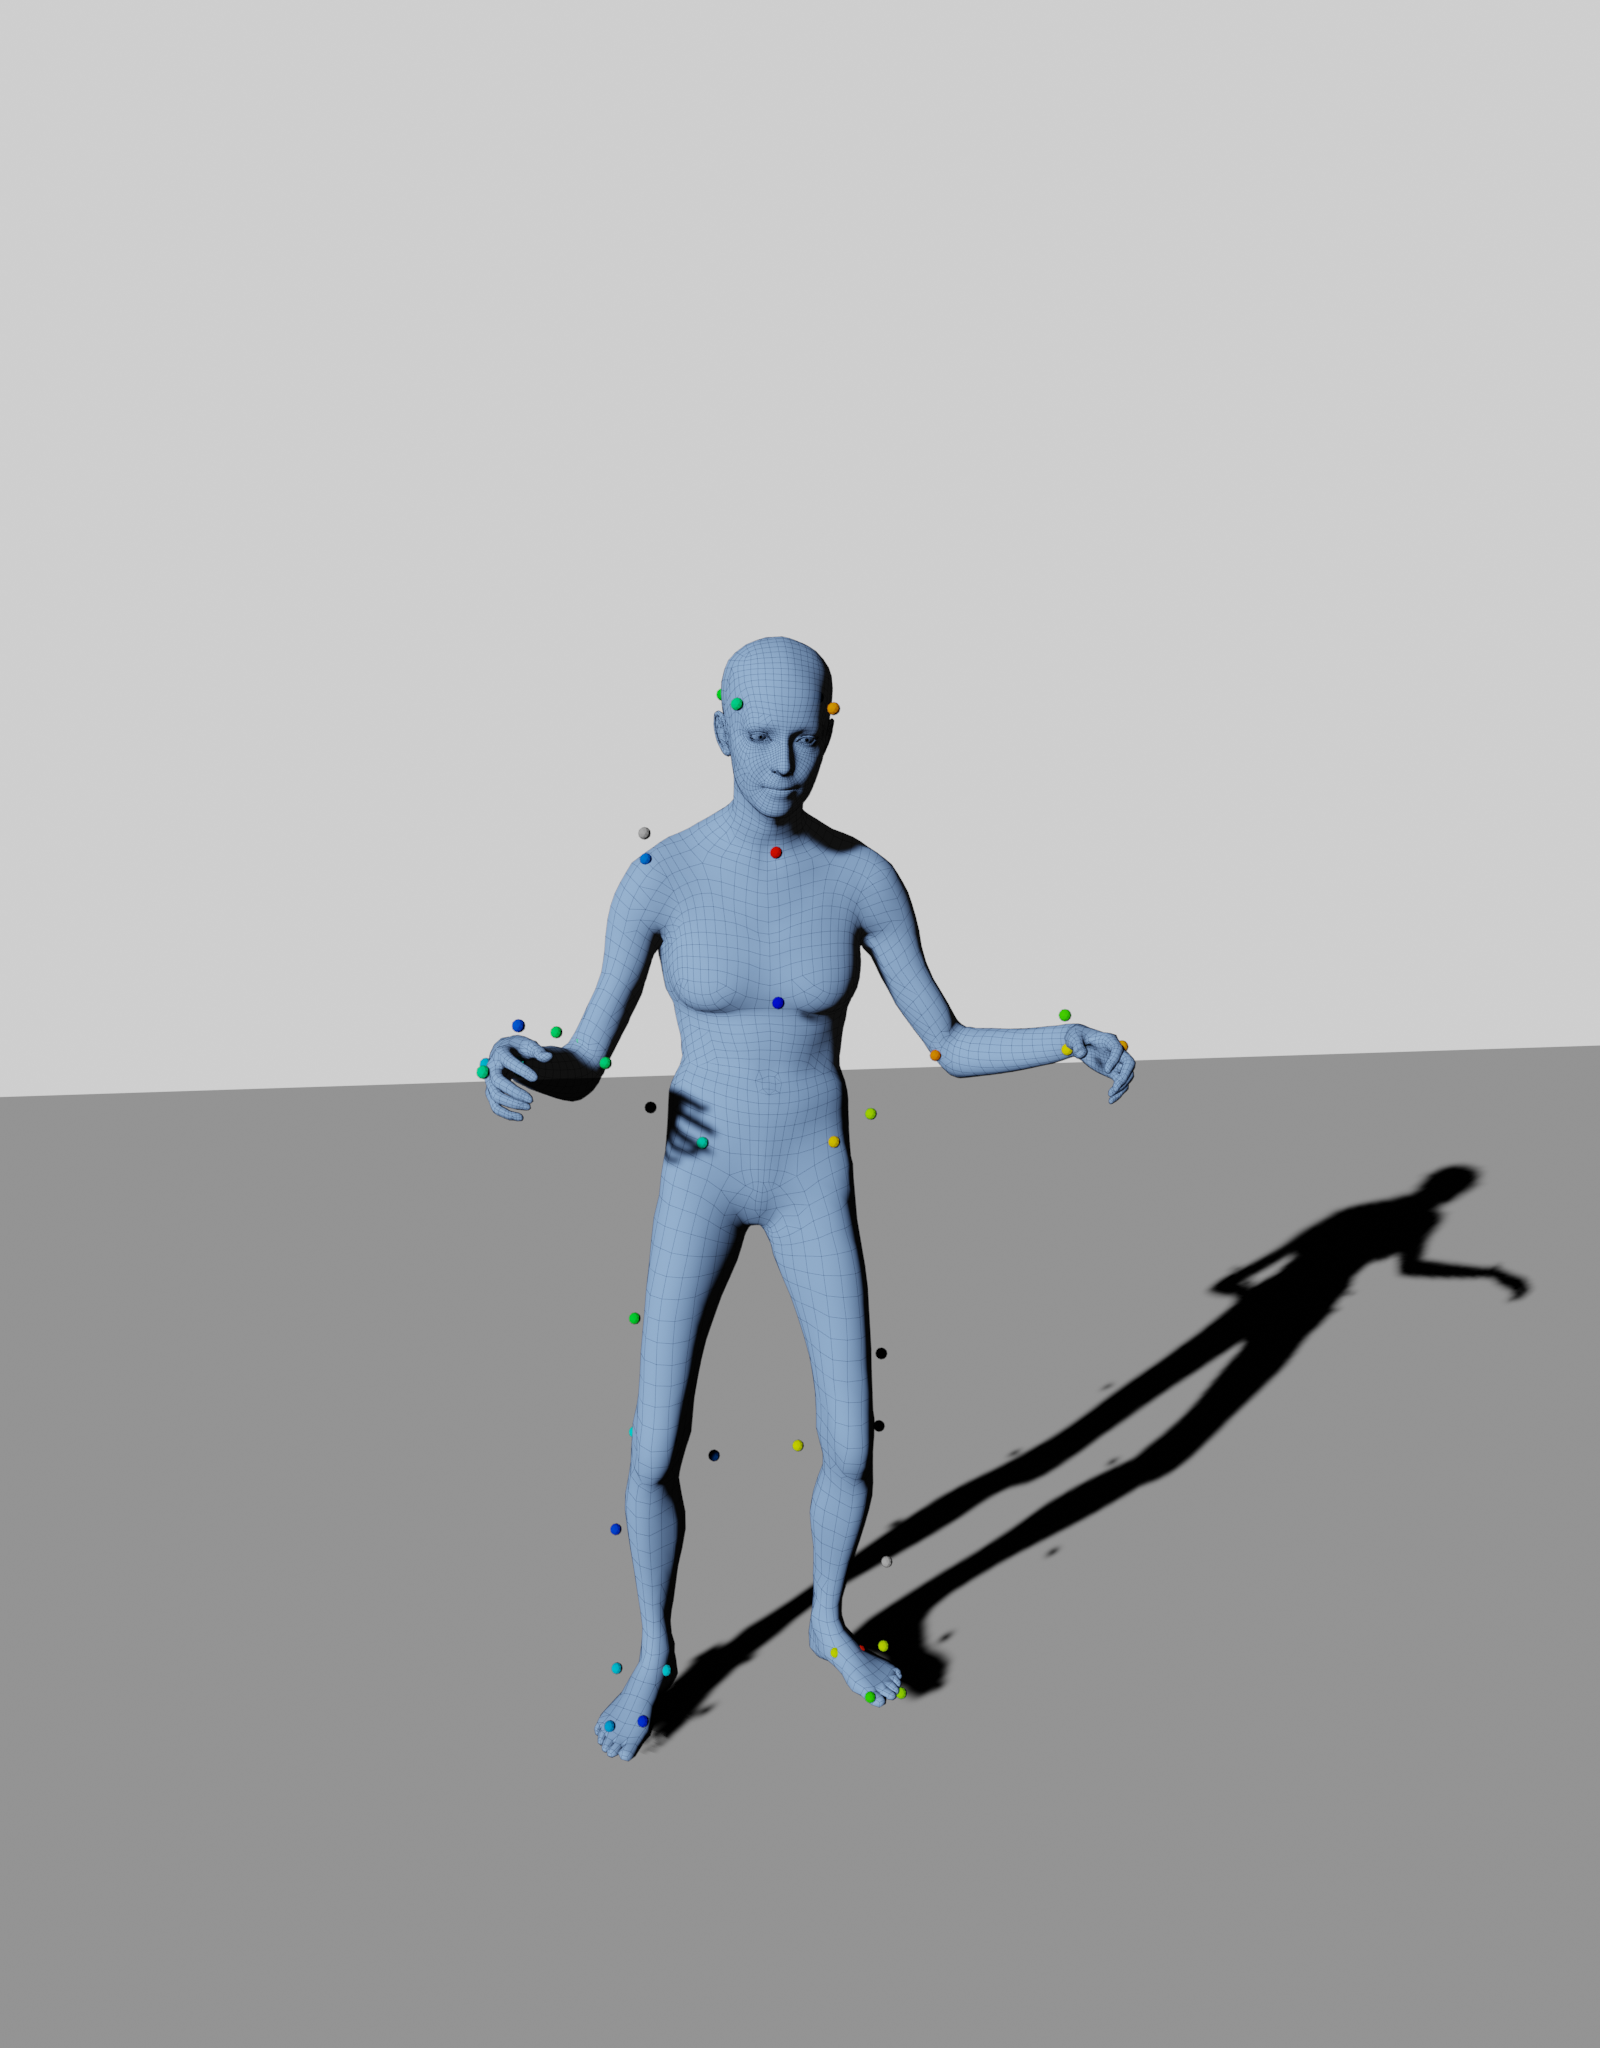
\includegraphics[width=0.48\textwidth]{figures/under.png}
        \label{fig:soma_initial}
    }
    \hfill % Adds horizontal space between the figures
    % Second subfigure
    \subfloat[Final solved mesh correct fit.]{
        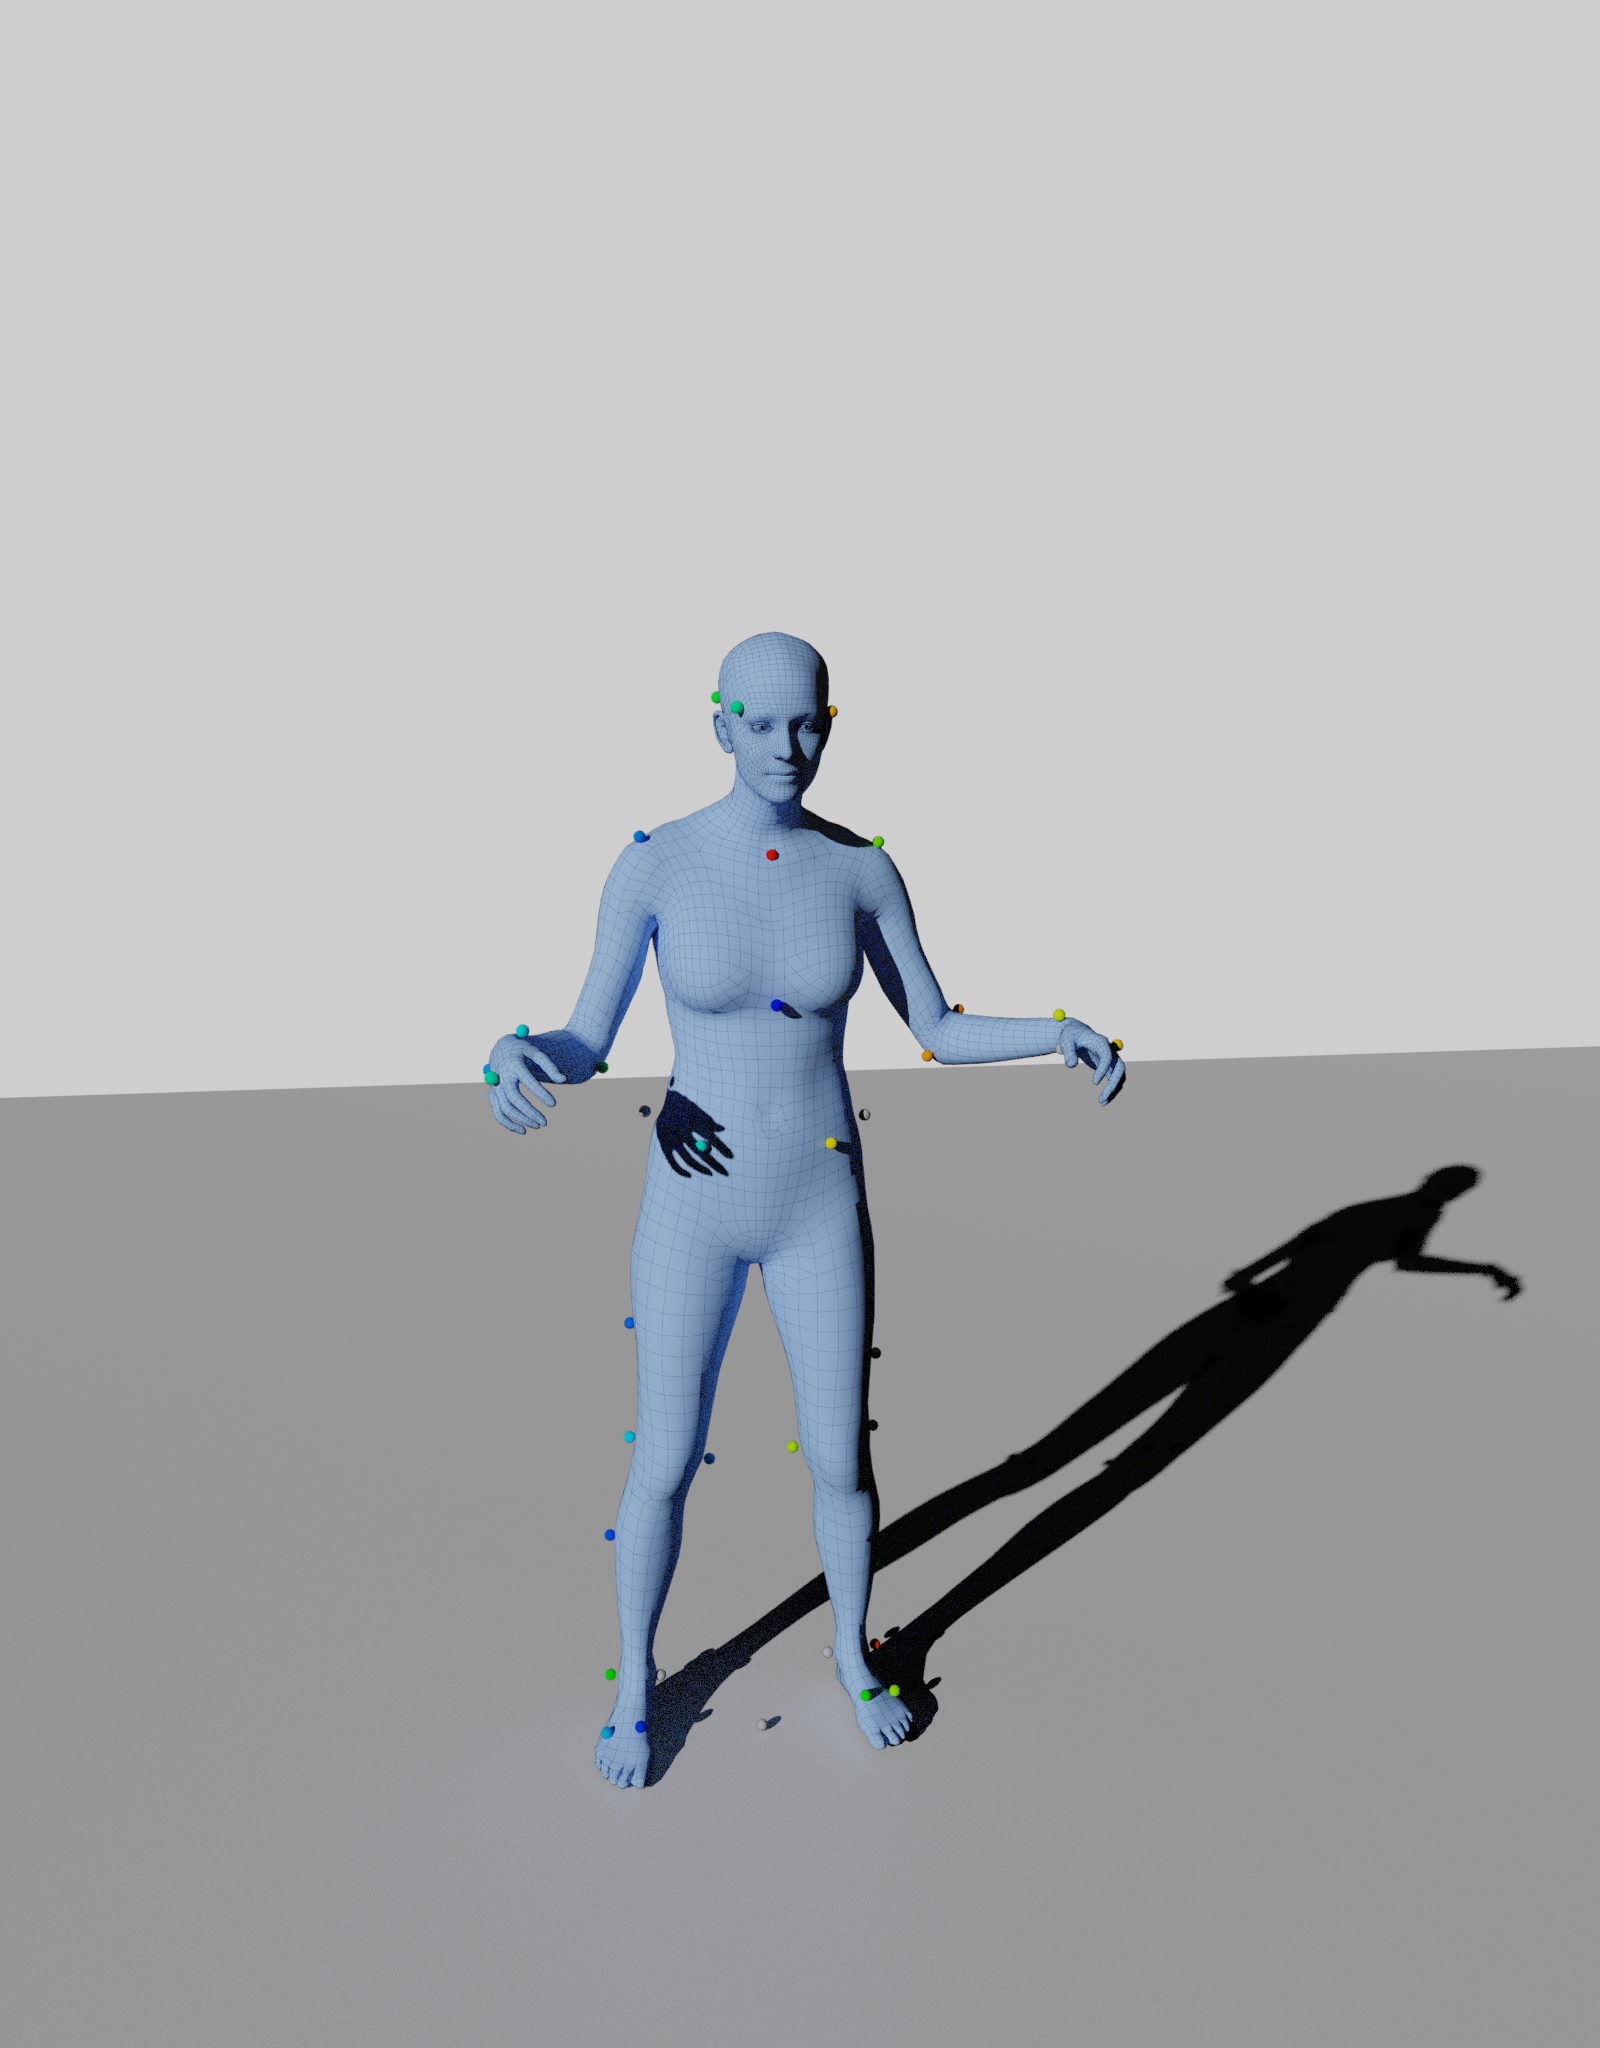
\includegraphics[width=0.48\textwidth]{figures/fit.png}
        \label{fig:soma_final}
    }
    \caption{Visual comparison of the SMPL-X mesh fitting process to the raw motion capture marker data.}
    \label{fig:soma_solve_comparison}
\end{figure}

\subsection{Importing SMPL-X into Blender}

Using the official Blender SMPL-X add-on \cite{SMPL-X:2019,tesch_smplx_blender_addon} we loaded in the .npz animation file.

\subsection{Motion Repair}

It is worth noting that despite the increased sampling rate and decrease in deformations some animation files still had deformations.

\subsection{Repetition Selection and Stitching}
% ARCHITECTURE.md 4

Using Blenders animation feature every start and end repetion frames were recorded. We are only interested in the precise human motion and kinematics for the exercise. We dp mpt consider the rest inbetween or the warm up. We decide that because we have 7 exercises we would stitch together the fastest 3 reps of each exercise to average out 
We then decided to stitch each subjects motion files together into a single sequence A3-A7 together. We took the 3 fastest reps from the fastest non-deformed human meshes so that we could average it out per action. We could've ysed inverse kinematics to smooth together the animation files so that it smoothly transistions from one animation file to the next but we are using non-temporal pose estimation algorithms. What is of most importance to us is representing realistic human motion data and getting renders. 
Having a subjects subsampled sequence from the dataset we stitched these togetheer.

Once we had procured human motion data in a sufficient format the next step is adding realism. 

\section{Human Body Model}
\label{sec:bodymodel}
% O2

\subsection{The SMPL-X Body Model}
\cite{loper2015smpl, SMPL-X:2019}

\subsection{Textures, Clothing and Materials}
% Suggested: \cite{black2023bedlam, tesch2025bedlam2}

Bedlam 2.0 made available a number of textures and materials from their B2 dataset. This included 100 Meshcapade skintextures comprised of 7 ethnicities, 50 female, 50 male, minimal clothing using a bald head scalp. In addition we used the clothing overlay textures. 
For our purposes we did not follow the full route of creating clothing assests using clothing software and rendering. We also did not add hair cards to our dataset but for our purpose of predicting the human shape and optimising the camera placement we saw the data as sufficient.

We used the Blender Python Script function to layer and blend the skin textures with clothing textures. Intiially for some clothing objects there was clothing tearing but we found a suitable subset of data that when wrapped around the SMPL-X body mesh would not reveal sensitive areas such as the arms and the crotch region.

After adding a skin-tone and texture of the human body we used Blenders Shader editor to increase the roughness and of the clothing and decreasing it for the skin to give a more realistic skin reflection to the light. This was done programmatically using the Blender Scripting but \ref{fig:shader_editor} displays the Blender UI
[INSERT: blended skin graphic]

\begin{figure}
    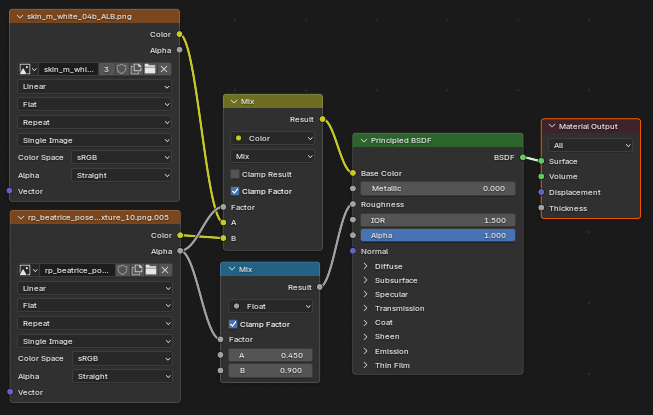
\includegraphics[width=0.48\textwidth]{figures/shader.png}
    \label{fig:shader_editor}
    \caption{Shader editor setup}
\end{figure}

\subsection{Subject Phenotypes}

\section{Camera Rig Design}
\label{sec:camerarig}
% O4. ARCHITECTURE.md 3

\subsection{Discretising the Configuration Space}
\cite{jorgensen2018simulation}

\subsection{Camera Model and Specifications}
% Suggested: \cite{schreuder2025sumedipose}

The choice of which cameras to utilise were informed by SUMediPose being chosen for the fact that they were realtively inexpensive and accessible meaning it does not require a specialised lab setup when one can use off the shelf cameras. The cameras chose were the Raspberry Pi Camera 3 module. 
The full spec sheet can be found at [insert: appendix/cite website] but table [insert table] displays the fov, sensor and lens properties.
Using Blender we configured the placement of the cameras based on these properties.

\subsection{Action Volume and Field-of-View Constraints}

A large choice needed some deep consideration which was the choice of camera placement and where to put them and how to structure the cameras and how many cameras are necessary.
We wanted to ensure that the cameras were as close to the human as possible but without cutting off any limbs whilst an action was being performed e.g lunges, jumping jacks or pushups.
A choice to create an Action Volume was made. Defining a region in which we knew the animated subject would be contained and confined to.
We decided that a cylindrical action volume best encompased the subject. We defined a a AV and radius of 1.5m height of 3.0m. With this defined object we used some math

Using the camera pproperties we programmatically checked if a particular placement and distance from a subject was valid. Using a Binary search approach we find the minimum safe distance, a distance from the subject such that the entire action volume is captured . 

\subsection{Ring Heights and Camera Distribution}

The dome fishbowl configuration starts with a total number of cameras how many layers there are and the minimum height and maximum height with a start and end pitch. Then using cosine curves using the number of rings and the start and end pitch the heights and pitches of the cameras to be placed are interporlated to workout the formulaic dome.

\subsection{Rig Radius}

Then based on the camera dome configuration each ring has a unique minimum safe distance that it can be placed from the action volume. This minimum safe disstance is calculated uisng the action volume and a binary search the camera placement is checked for validity using trignometric field of view calculations. Then for every ring in the camer configuration the are placed such that they look inward toward the origin and at a z-height of 1.5m fixed. This allows some padding and that if the subject jumps with the fov that equates to a max height of [insert: do calculation] with some padding for our subjects.

Images of the camera layout can be seen here [insert cameralayout diagram and maps]

We chose vertical, portrait orientations as we wanted to get the cameras as close to the subject as possible instead of being limited by a shorter fov in a landscape orientation.

\subsection{Camera Indexing and Orientation Convention}
% Camera number -> ring and yaw; yaw 0 = subject's front (FEPSO_RESULTS.md 1)

\section{Rendering}
\label{sec:rendering}
% ARCHITECTURE.md 5

\subsection{Render Engine and Settings}

We used EEVEE rendering withing Blender environment due to the trade off between realism and render time when compared to render times for Cycles rendering. 
We went frame by frame and camera by camera and subject by subject such that each camera would render out frame 0 for all subjects before going on to the next camera.
We used a Volume Light Probe to assist with light calculations to save on rendering time.

\subsection{Render Environment}

We used a clean render environment stripped down from a BlendKit environment. Constructed and adjusted to be as simple as possible for the base calculation.

\subsection{Parallel Headless Rendering}

\subsection{Subject Isolation}

\subsection{Frame Sampling and Storage}

we rendered out at a sub sampling of every second frame to both save time on rendering as this gives sufficient information and representation of the motion being performed

\subsection{Render Throughput}

\section{Ground Truth Extraction}
\label{sec:groundtruth}

\subsection{3D Joint Positions}
\cite{needham2021accuracy, patel2021agora}

\subsection{Camera Projection Matrices}
% ARCHITECTURE.md 3 (Matrices)

\subsection{Coordinate Systems and Units}

\section{2D Human Pose Estimation}
\label{sec:inference}
% Implements O7; the model comparison itself is in Chapter~\ref{chap:results}. ARCHITECTURE.md 6
% TODO bib: YOLO26 (Ultralytics), HRNet, ViTPose, MMPose, COCO keypoints

\subsection{Pose Estimation Models}

Inference there are many pose estimation algorithms to work with ViTPose, HRnet, OpenPose, YoloPose, MediaPipe.  

\subsection{Shared Detection and Matched Crops}

\subsection{Keypoint Format and Scored Joints}

\subsection{Concurrent Rendering and Inference}

\subsection{Batched Inference and Verification}

\section{Resulting Dataset}
\label{sec:dataset}
% FEPSO_RESULTS.md 1; ARCHITECTURE.md 4, 6

\subsection{Composition}

\subsection{Keypoint Storage and Labels}

\section{Chapter Summary}
\label{sec:pipelinesummary}
